% \fs and \fmax must be defined before calling this picture.
\def\fs{10}
\def\fmax{5}
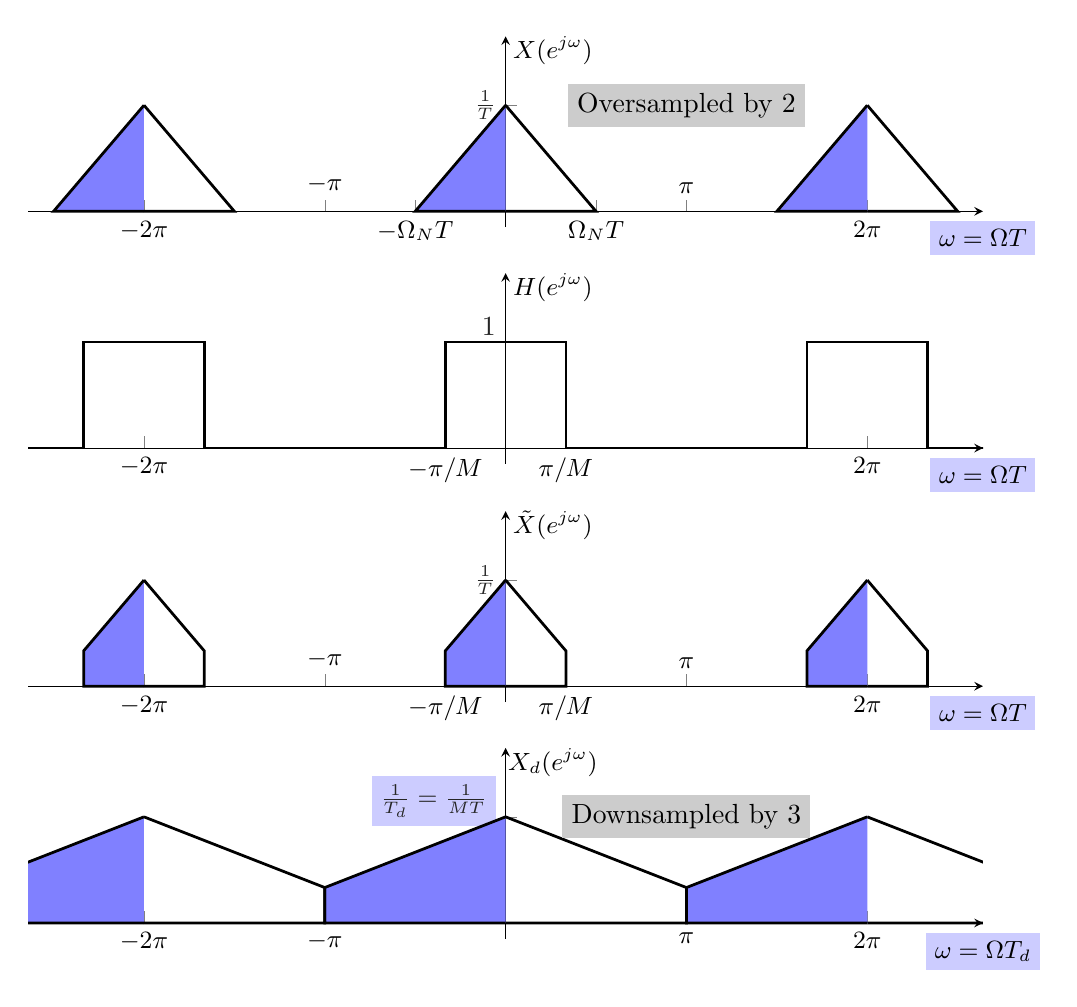
\begin{tikzpicture}
\onslide<1-|handout:1>{
\begin{axis}[
	name=plot1,
	axis lines*=middle,
	enlargelimits = true,
	clip=true,
	scale only axis,
	width=\textwidth,
	height=0.2\textwidth,
	ymin=0,
	ymax=3,
	xmin=-\fs-1,
	xmax=\fs+1,
	axis line style={->,>=stealth},
	xlabel={\small \tikz[baseline]{\node[fill=blue!20,anchor=base] (t1) {$\omega = \Omega T$};}},
	ylabel={\small $X(e^{j\omega})$},
	every axis x label/.style={
		at={(ticklabel* cs:1)},
		%xshift=0.2cm,
		anchor=north,
	},
	every axis y label/.style={
		at={(ticklabel* cs:0.8)},
		anchor=south,
		xshift=0.6cm,
	},
	xtick=\empty,
	ytick=2,
	yticklabels={\small $\frac{1}{T}$},
	xtick={-\fs, -2.5, 0, 2.5, \fs},
	xticklabels={\small $-2\pi$, \small $-\Omega_NT$, \small 0, \small $\Omega_NT$, \small $2\pi$}, 
	extra x ticks={-\fmax, \fmax},
	extra x tick labels={\small $-\pi$, \small $\pi$},
	extra x tick style={
		xticklabel style={yshift=0.7ex, anchor=south}
	},
	every outer y axis line/.append style={white!15!black},
	every y tick label/.append style={font=\color{white!15!black}},
	legend style={draw=white!15!black,fill=white,legend cell align=left}]
	\addplot[solid, line width=1pt] coordinates {(0, 2) (2.5, 0) (0, 0)};
	\addplot[solid, line width=1pt, fill=blue!50] coordinates {(0, 2) (-2.5, 0) (0, 0)};
	\addplot[solid, line width=1pt] coordinates {(\fs, 2) (\fs+2.5, 0) (\fs, 0)};
	\addplot[solid, line width=1pt, fill=blue!50] coordinates {(\fs, 2) (\fs-2.5, 0) (\fs, 0)};
	\addplot[solid, line width=1pt] coordinates {(-\fs, 2) (-\fs+2.5, 0) (-\fs, 0)};
	\addplot[solid, line width=1pt, fill=blue!50] coordinates {(-\fs, 2) (-\fs-2.5, 0) (-\fs, 0)};
	\addplot[solid, line width=1pt] coordinates {(-2*\fs, 2) (-2*\fs+2.5, 0) (-2*\fs, 0)};
	\addplot[solid, line width=1pt, fill=blue!50] coordinates {(-2*\fs, 2) (-2*\fs-2.5, 0) (-2*\fs, 0)};]
	\addplot[solid, line width=1pt] coordinates {(2*\fs, 2) (2*\fs+2.5, 0) (2*\fs, 0)};
	\addplot[solid, line width=1pt, fill=blue!50] coordinates {(2*\fs, 2) (2*\fs-2.5, 0) (2*\fs, 0)};
	\node[scale=1, fill=black!20] at (axis cs: 5, 2) {Oversampled by 2};
\end{axis}
}
\def\fbw{1.6667}
\def\fint{0.6667}
\onslide<2-|handout:1>{
\begin{axis}[
	name=plot2,
	at=(plot1.below south east), anchor=above north east,
	axis lines*=middle,
	enlargelimits = true,
	clip=true,
	scale only axis,
	width=\textwidth,
	height=0.2\textwidth,
	ymin=0,
	ymax=3,
	xmin=-\fs-1,
	xmax=\fs+1,
	axis line style={->,>=stealth},
	xlabel={\small \tikz[baseline]{\node[fill=blue!20,anchor=base] (t1) {$\omega = \Omega T$};}},
	ylabel={\small $H(e^{j\omega})$},
	every axis x label/.style={
		at={(ticklabel* cs:1)},
		%xshift=0.2cm,
		anchor=north,
	},
	every axis y label/.style={
		at={(ticklabel* cs:0.8)},
		anchor=south,
		xshift=0.6cm,
	},
	xtick=\empty,
	ytick=2,
	yticklabels={1},
	yticklabel style={yshift=0.2cm},
	xtick={-\fs, -\fbw, \fbw, \fs},
	xticklabels={\small $-2\pi$, \small $-\pi/M$, \small $\pi/M$, \small $2\pi$}, 
	every outer y axis line/.append style={white!15!black},
	every y tick label/.append style={font=\color{white!15!black}},
	legend style={draw=white!15!black,fill=white,legend cell align=left}]
	\addplot[solid, line width=1pt] coordinates {(-2*\fs-\fbw, 0) (-2*\fs-\fbw, 2) (-2*\fs+\fbw, 2) (-2*\fs+\fbw, 0) (-\fs-\fbw, 0) (-\fs-\fbw, 2) (-\fs+\fbw, 2) (-\fs+\fbw, 0)  (-\fbw, 0) (-\fbw, 2) (\fbw, 2) (\fbw, 0) (\fs-\fbw, 0) (\fs-\fbw, 2) (\fs+\fbw, 2) (\fs+\fbw, 0) (2*\fs-\fbw, 0)};
\end{axis}
}
\onslide<3-|handout:1>{
\begin{axis}[
	name=plot3,
	at=(plot2.below south east), anchor=above north east,
	axis lines*=middle,
	enlargelimits = true,
	clip=true,
	scale only axis,
	width=\textwidth,
	height=0.2\textwidth,
	ymin=0,
	ymax=3,
	xmin=-\fs-1,
	xmax=\fs+1,
	axis line style={->,>=stealth},
	xlabel={\small \tikz[baseline]{\node[fill=blue!20,anchor=base] (t1) {$\omega = \Omega T$};}},
	ylabel={\small $\tilde{X}(e^{j\omega})$},
	every axis x label/.style={
		at={(ticklabel* cs:1)},
		%xshift=0.2cm,
		anchor=north,
	},
	every axis y label/.style={
		at={(ticklabel* cs:0.8)},
		anchor=south,
		xshift=0.6cm,
	},
	xtick=\empty,
	ytick=2,
	yticklabels={\small $\frac{1}{T}$},
	xtick={-\fs, -\fbw, \fbw, \fs},
	xticklabels={\small $-2\pi$, \small $-\pi/M$, \small $\pi/M$, \small $2\pi$}, 
	extra x ticks={-\fmax, \fmax},
	extra x tick labels={\small $-\pi$, \small $\pi$},
	extra x tick style={
		xticklabel style={yshift=0.7ex, anchor=south}
	},
	every outer y axis line/.append style={white!15!black},
	every y tick label/.append style={font=\color{white!15!black}},
	legend style={draw=white!15!black,fill=white,legend cell align=left}]
	\addplot[solid, line width=1pt] coordinates {(0, 2) (\fbw, \fint) (\fbw, 0) (0, 0)};
	\addplot[solid, line width=1pt, fill=blue!50] coordinates {(0, 2) (-\fbw, \fint) (-\fbw, 0) (0, 0)};
	\addplot[solid, line width=1pt] coordinates {(-\fs, 2) (\fbw-\fs, \fint) (\fbw-\fs, 0) (-\fs, 0)};
	\addplot[solid, line width=1pt, fill=blue!50] coordinates {(-\fs, 2) (-\fbw-\fs, \fint) (-\fbw-\fs, 0) (-\fs, 0)};
	\addplot[solid, line width=1pt] coordinates {(\fs, 2) (\fs+\fbw, \fint) (\fs+\fbw, 0) (\fs, 0)};
	\addplot[solid, line width=1pt, fill=blue!50] coordinates {(\fs, 2) (\fs-\fbw, \fint) (\fs-\fbw, 0) (\fs, 0)};
\end{axis}
}
\def\fbw{5}
\def\fint{0.6667}
\onslide<4|handout:1>{
\begin{axis}[
	name=plot4,
	at=(plot3.below south east), anchor=above north east,
	axis lines*=middle,
	enlargelimits = true,
	clip=true,
	scale only axis,
	width=\textwidth,
	height=0.2\textwidth,
	ymin=0,
	ymax=3,
	xmin=-\fs-1,
	xmax=\fs+1,
	axis line style={->,>=stealth},
	xlabel={\small \tikz[baseline]{\node[fill=blue!20,anchor=base] (t1) {$\omega = \Omega T_d$};}},
	ylabel={\small $X_d(e^{j\omega})$},
	every axis x label/.style={
		at={(ticklabel* cs:1)},
		%xshift=0.2cm,
		anchor=north,
	},
	every axis y label/.style={
		at={(ticklabel* cs:0.8)},
		anchor=south,
		xshift=0.6cm,
	},
	xtick=\empty,
	ytick=2,
	yticklabels={\small \tikz[baseline]{\node[fill=blue!20,anchor=base] {$\frac{1}{T_d} = \frac{1}{MT}$};}},
	yticklabel style={yshift=0.2cm},
	xtick={-\fs, -\fbw, \fbw, \fs},
	xticklabels={\small $-2\pi$, \small $-\pi$, \small $\pi$, \small $2\pi$}, 
	every outer y axis line/.append style={white!15!black},
	every y tick label/.append style={font=\color{white!15!black}},
	legend style={draw=white!15!black,fill=white,legend cell align=left}]
	\addplot[solid, line width=1pt] coordinates {(0, 2) (\fbw, \fint) (\fbw, 0) (0, 0)};
	\addplot[solid, line width=1pt, fill=blue!50] coordinates {(0, 2) (-\fbw, \fint) (-\fbw, 0) (0, 0)};
	\addplot[solid, line width=1pt] coordinates {(-\fs, 2) (\fbw-\fs, \fint) (\fbw-\fs, 0) (-\fs, 0)};
	\addplot[solid, line width=1pt, fill=blue!50] coordinates {(-\fs, 2) (-\fbw-\fs, \fint) (-\fbw-\fs, 0) (-\fs, 0)};
	\addplot[solid, line width=1pt] coordinates {(\fs, 2) (\fs+\fbw, \fint) (\fs+\fbw, 0) (\fs, 0)};
	\addplot[solid, line width=1pt, fill=blue!50] coordinates {(\fs, 2) (\fs-\fbw, \fint) (\fs-\fbw, 0) (\fs, 0)};
	\node[scale=1, fill=black!20] at (axis cs: 5, 2) {Downsampled by 3};
\end{axis}
}
\end{tikzpicture}
